\documentclass{article} % For LaTeX2e
\usepackage{nips13submit_e,times}
\usepackage{hyperref}
\usepackage{url}
\usepackage{authblk}
\usepackage{graphicx}
\usepackage[numbers]{natbib}
\usepackage{amsmath}

%\documentstyle[nips13submit_09,times,art10]{article} % For LaTeX 2.09

\begin{document}

\title{Investigation of Machine Learning Techniques with Application to the SVHN Dataset
\author{Bai, Min \texttt{mbai@cs.toronto.edu}}
\author{Loyzer, Mark \texttt{loyzer@cs.toronto.edu}}
\affil{Department of Computer Science
University of Toronto
Toronto, Ontario, Canada}
}

\newcommand{\fix}{\marginpar{FIX}}
\newcommand{\new}{\marginpar{NEW}}

\nipsfinalcopy % Uncomment for camera-ready version

\maketitle

\section{Introduction}
This project focuses on classifying digits from street view images.  We use the Street View House Numbers dataset from \cite{svhn}. All images have a fixed 32x32 resolution with character-level ground truth labels. For each example, the labelled character is centered at the image. Since this is a digit recognition task there are ten classes in total.

The data is collected from street-view images, thus there exist vast intra-class variations (varying fonts, colours, etc). To generate competitive performance, we have considered a variety of classification techniques exploiting feature representations that are robust to intra-class variations. We attempt both hand-crafted and learned features as well as raw pixel data as the purpose of this project is to investigate different machine learning techniques and so knowing the pitfalls and prevalences of each technique. The specific techniques we attempt are neural networks (specifically, convolutional neural networks, K-nearest neighbours, and support vector machines).  We describe the setup, performance, results, and summarize the investigation for each of the techniques.

\section{Convolutional Neural Networks}

\subsection{Setup}

The first method we explored is the convolutional neural networks technique. The architectures explored are based on a 2012 CVPR paper \cite{lecun2012}, as well as the tutorials provided by Google in their Tensorflow tutorials \cite{googletensorflow}. 

The basic structure of the network consists of several convolution layers followed by several fully connected layers, which finally finally feed to a 10 unit softmax output. The details of these layers is discussed in the following sections. 

\subsubsection{Convolution Layer}

The standard convolution layer consists of a 2 dimensional patch of size 5x5. The layer takes in M input feature channels, and produces N output feature channels by through parallelism. The convolution operation is described by the following equation. 

\begin{gather}
{h_{i,j,n}}^l = \sigma(\sum_{e=1}^{M}{\sum_{a=-2}^{2}{\sum_{b=-2}^{2} w_{a,b,m,n}h_{(i+a),(i+b),m}^{l-1}} + b_n}) \\
\sigma(x) = \text{max}\{0, x\}
\end{gather}

where ${h_{i,j,n}}^l$ is the (i,j)-th indexed output in the l-th layer in channel n, while $w_{a,b,m,n}$ is a weight in the convolution layer, and $b_n$ the bias value for the n-th output layer. 

\subsubsection{Local Response Normalization Layer}

The local response normalization layer is akin to a image whitening, whereby the input to the next layer is rescaled so that the nearby neurons receive input of roughly the same size. This can theoretically improve training performance. 

\subsubsection{Pooling Layer} 

Max pooling is used to reduce the size of the image, and to provide some shift invariance. Since we are only attempting to detect one number in the input image, the use of max pooling allows us to find the area with the maximum response. The pooling function operates over a 2x2 square, and returns the maximum value among the 4 values in the square. Moreover, the pooling scheme has a stride size of 2, effectively having no overlap. It has been shown that pooling can contribute significantly to object recognition based on convolutional neural networks \cite{pooling}, and it is hoped that it will be useful for digit recognition as well. 

\subsubsection{Fully Connected Layer}

The fully connected layers are used at the output of the neural network. This is the standard neuron, with every neuron connected to all neurons in the preceding and following layer. The model is as follows:

\begin{gather}
{h_{j}}^l = \sigma({w_{i,j}}^{l} {h_{i}}^{l-1} + {b_j}^l) 
\end{gather}

\subsubsection{Implementation and Training}

Various configurations using the preceding network layers are instantiated using the Google TensorFlow package. The network is then optimized using the built in AdamOptimizer, with the cross entropy as the cost function to be minimized:

\begin{gather}
J(w) = - \sum_{i}{\sum_{k=0}^{9}{t^{(i)}_k}log(y_k(x^{(i)}))}
\end{gather}

where t are the one-hot targets, and y is the the output vector of the final multi-class softmax function. 

Mini-batch training is used to train the neural networks, with 50 input samples per batch. These mini-batches are selected at random with replacement from the sample set. Both the training and extra-training input images from the SVHN website are used, for a total of 604388 training samples. Because of the large quantity of test data available (26032 samples, which is on average 2600 samples per digit), we decided to use 10000 of these for the validation set, and the remaining 16032 for the test set to obtain an unbiased estimate of the performance of our implementation.

Through experimentation, it is found that initializing the weights and biases with a Gaussian distribution of zero mean and standard deviation of 0.05 resulted in the training sequences where the gradient does not explode during early training. 

For each neural network configuration, training is done until the validation error (evaluated every 1000 epochs) becomes roughly constant. The weights are saved every 10000 epochs as checkpoints. The weights from the iteration where the validation error is minimum are used to obtain an evaluation for the final test set evaluation. 

\subsection{Configurations and Results}

The configurations of convolutional neural networks tested are listed in the Table \ref{networkcfgs}. 

\begin{table}[h]
\centering
\caption{Network Configurations Explored}
\label{networkcfgs}
\resizebox{\textwidth}{!}{
\begin{tabular}{llllllll}
\hline
\multicolumn{1}{|l|}{Layer}                 & \multicolumn{1}{l|}{Config 1}    & \multicolumn{1}{l|}{Config 2}     & \multicolumn{1}{l|}{Config 3}    & \multicolumn{1}{l|}{Config 4}    & \multicolumn{1}{l|}{Config 5}    & \multicolumn{1}{l|}{Config 6}    & \multicolumn{1}{l|}{Config 7}    \\ \hline
\multicolumn{1}{|l|}{Convolution 1}         & \multicolumn{1}{l|}{5x5, 3, 32}  & \multicolumn{1}{l|}{5x5, 3, 32}   & \multicolumn{1}{l|}{5x5, 3, 32}  & \multicolumn{1}{l|}{5x5, 3, 64}  & \multicolumn{1}{l|}{5x5, 3, 32}  & \multicolumn{1}{l|}{5x5, 3, 32}  & \multicolumn{1}{l|}{5x5, 3, 32}  \\ \hline
\multicolumn{1}{|l|}{Pooling 1}             & \multicolumn{1}{l|}{yes}         & \multicolumn{1}{l|}{no}           & \multicolumn{1}{l|}{yes}         & \multicolumn{1}{l|}{yes}         & \multicolumn{1}{l|}{yes}         & \multicolumn{1}{l|}{yes}         & \multicolumn{1}{l|}{yes}         \\ \hline
\multicolumn{1}{|l|}{Local Response Norm 1} & \multicolumn{1}{l|}{no}          & \multicolumn{1}{l|}{no}           & \multicolumn{1}{l|}{yes}         & \multicolumn{1}{l|}{no}          & \multicolumn{1}{l|}{no}          & \multicolumn{1}{l|}{no}          & \multicolumn{1}{l|}{no}          \\ \hline
                                            &                                  &                                   &                                  &                                  &                                  &                                  &                                  \\ \hline
\multicolumn{1}{|l|}{Convolution 2}         & \multicolumn{1}{l|}{5x5, 32, 64} & \multicolumn{1}{l|}{5x5, 32, 64}  & \multicolumn{1}{l|}{5x5, 32, 64} & \multicolumn{1}{l|}{5x5, 64, 64} & \multicolumn{1}{l|}{5x5, 32, 64} & \multicolumn{1}{l|}{5x5, 32, 64} & \multicolumn{1}{l|}{5x5, 32, 64} \\ \hline
\multicolumn{1}{|l|}{Pooling 2}             & \multicolumn{1}{l|}{yes}         & \multicolumn{1}{l|}{yes}          & \multicolumn{1}{l|}{yes}         & \multicolumn{1}{l|}{no}          & \multicolumn{1}{l|}{no}          & \multicolumn{1}{l|}{no}          & \multicolumn{1}{l|}{no}          \\ \hline
\multicolumn{1}{|l|}{Local Response Norm 2} & \multicolumn{1}{l|}{no}          & \multicolumn{1}{l|}{no}           & \multicolumn{1}{l|}{yes}         & \multicolumn{1}{l|}{no}          & \multicolumn{1}{l|}{no}          & \multicolumn{1}{l|}{no}          & \multicolumn{1}{l|}{no}          \\ \hline
                                            &                                  &                                   &                                  &                                  &                                  &                                  &                                  \\ \hline
\multicolumn{1}{|l|}{Convolution 3}         & \multicolumn{1}{l|}{no}          & \multicolumn{1}{l|}{no}           & \multicolumn{1}{l|}{no}          & \multicolumn{1}{l|}{5x5, 64, 64} & \multicolumn{1}{l|}{5x5, 32, 64} & \multicolumn{1}{l|}{5x5, 32, 64} & \multicolumn{1}{l|}{5x5, 32, 64} \\ \hline
\multicolumn{1}{|l|}{Pooling 3}             & \multicolumn{1}{l|}{no}          & \multicolumn{1}{l|}{no}           & \multicolumn{1}{l|}{no}          & \multicolumn{1}{l|}{yes}         & \multicolumn{1}{l|}{yes}         & \multicolumn{1}{l|}{yes}         & \multicolumn{1}{l|}{no}          \\ \hline
\multicolumn{1}{|l|}{Local Response Norm 3} & \multicolumn{1}{l|}{no}          & \multicolumn{1}{l|}{no}           & \multicolumn{1}{l|}{no}          & \multicolumn{1}{l|}{no}          & \multicolumn{1}{l|}{no}          & \multicolumn{1}{l|}{no}          & \multicolumn{1}{l|}{no}          \\ \hline
                                            &                                  &                                   &                                  &                                  &                                  &                                  &                                  \\ \hline
\multicolumn{1}{|l|}{Convolution 4}         & \multicolumn{1}{l|}{no}          & \multicolumn{1}{l|}{no}           & \multicolumn{1}{l|}{no}          & \multicolumn{1}{l|}{no}          & \multicolumn{1}{l|}{no}          & \multicolumn{1}{l|}{no}          & \multicolumn{1}{l|}{5x5, 32, 64} \\ \hline
\multicolumn{1}{|l|}{Pooling 4}             & \multicolumn{1}{l|}{no}          & \multicolumn{1}{l|}{no}           & \multicolumn{1}{l|}{no}          & \multicolumn{1}{l|}{no}          & \multicolumn{1}{l|}{no}          & \multicolumn{1}{l|}{no}          & \multicolumn{1}{l|}{yes}         \\ \hline
\multicolumn{1}{|l|}{Local Response Norm 4} & \multicolumn{1}{l|}{no}          & \multicolumn{1}{l|}{no}           & \multicolumn{1}{l|}{no}          & \multicolumn{1}{l|}{no}          & \multicolumn{1}{l|}{no}          & \multicolumn{1}{l|}{no}          & \multicolumn{1}{l|}{no}          \\ \hline
                                            &                                  &                                   &                                  &                                  &                                  &                                  &                                  \\ \hline
\multicolumn{1}{|l|}{Fully Connected 1}     & \multicolumn{1}{l|}{4096 x 1024} & \multicolumn{1}{l|}{16384 x 1024} & \multicolumn{1}{l|}{4096 x 1024} & \multicolumn{1}{l|}{4096 x 1024} & \multicolumn{1}{l|}{4096 x 1024} & \multicolumn{1}{l|}{4096x2048}   & \multicolumn{1}{l|}{4096 x 1024} \\ \hline
                                            &                                  &                                   &                                  &                                  &                                  &                                  &                                  \\ \hline
\multicolumn{1}{|l|}{Fully Connected 2}     & \multicolumn{1}{l|}{1024 x 10}   & \multicolumn{1}{l|}{1024 x 10}    & \multicolumn{1}{l|}{1024 x 10}   & \multicolumn{1}{l|}{1024 x 10}   & \multicolumn{1}{l|}{1024 x 10}   & \multicolumn{1}{l|}{2048x10}     & \multicolumn{1}{l|}{1024 x 10}   \\ \hline
\end{tabular}}
\end{table}

The training progression is shown in Figure \ref{convplot}. Note that the configurations are as labelled in Table \ref{networkcfgs}. It is noteworthy that the training progress tends to level out after about 80000 epochs. Moreover, it is important to note that for several configurations, the training ended abruptly before reaching the end due to some gradients having exceeded pre-set size boundaries. However, this appeared to only occur when the validation error has stopped improving, and hence should not impact the selection of a good set of weights. 

\begin{figure}[h]
\caption{Training Progress}
\label{convplot}
\centering
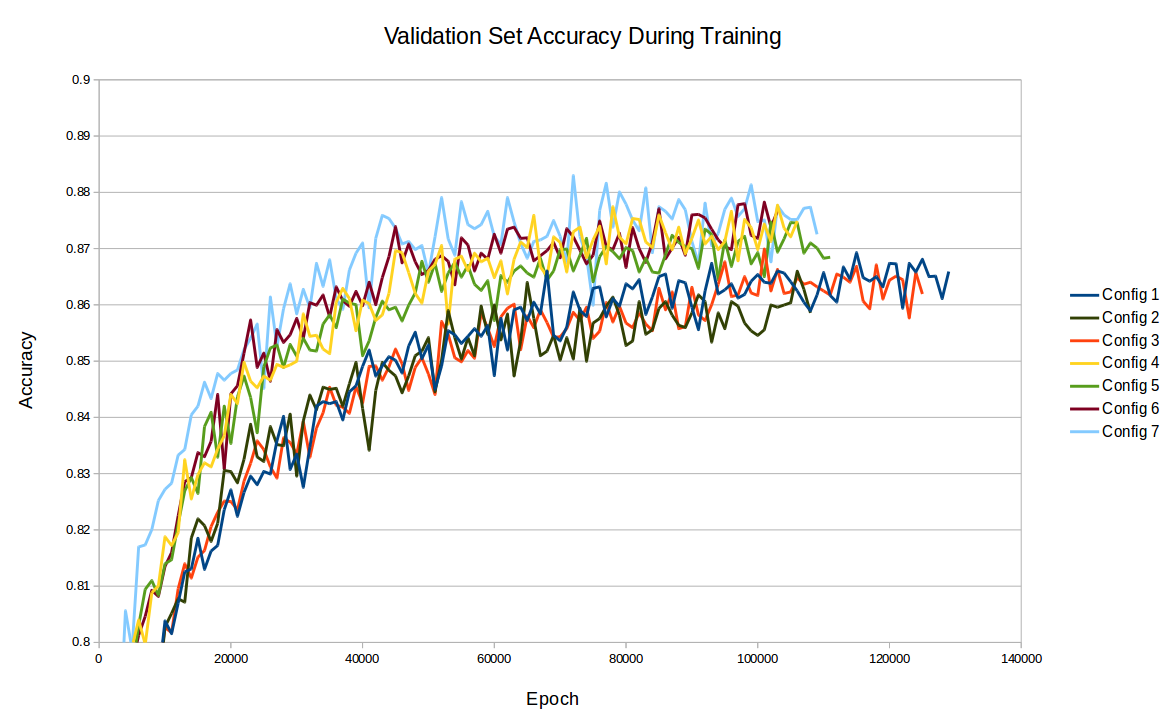
\includegraphics[width=1\textwidth]{plots/convplot}
\end{figure}

The final test set accuracies of the various configurations are shown in the table below. 

\begin{table}[h]
\centering
\caption{Test Set Accuracies}
\label{convtest}
\resizebox{\textwidth}{!}{
\begin{tabular}{|l|l|l|l|l|l|l|l|}
\hline
                  & Config 1 & Config 2 & Config 3 & Config 4 & Config 5 & Config 6 & Config 7 \\ \hline
Test Set Accuracy & 0.851    & 0.844    & 0.849    & 0.862    & 0.861    & 0.857    & 0.863    \\ \hline
\end{tabular}}
\end{table}


\subsection{Discussions}

There are numerous observations we can make from the results in Table \ref{convtest}. 

\subsubsection{Pooling}

Configuration 1 and Configuration 2 differ in the presence and absence of a max pooling layer that operates over non-overlapping 2x2 patches, respectively. In Configuration 1, there is one such layer after both the first and the second convolution layers, while in Configuration 2, there is only one such layer after the second convolution layer. 

Configuration 1 obtained 85.1\% accuracy on the test set, while Configuration 2 obtained 84.4\% accuracy. Moreover, the validation set error toward the end of the training also appears to be lower for Configuration 2. We can conclude that the pooling layer has an impact on our results. 

\subsubsection{}

\section{K-Nearest Neighbours}
K-Nearest Neighbours (K-NN) has traditionally performed very well in a variety of tasks so we investigated the performance of K-NN in the SVHN domain.

\subsection{Setup}
Using the raw pixel data ($32 x 32 x 3 = 3072$ dimensions) was too time intensive and so PCA was used to reduce the dimensionality to make the computations more feasible.  The PCA dimension space was determined through cross-validation as well as inspecting the eigenvector weights to determine the significance each eigenvector had for preserving the information contained in the dataset (see Section~\ref{knn_pca} for the direct analysis on top PCA dimensions).  Additionally, the number of neighbours to consider when determining the class for a new example (K hyper-parameter) was also determined using cross validation.  We used two variations of K-NN: the canonical voting rule where each of the top K classes have equal weight in deciding the predicted class and the inverse-weight function so that closer examples had a greater influence on the predicted class. We use the L2-Norm for our distance metric as it is the more canonical metric though others could be used as well. Due to memory limitations only the 'train\_32x32' and 'test\_32x32' datasets were used for training and validating the model respectively.

\subsection{Determining PCA Dimension} \label{knn_pca}
The top 20 eigenvector weights were: [0.58293515, 0.05988745, 0.05289433, 0.04385749, 0.02023858, 0.01697088, 0.01630875, 0.01405416, 0.01276369, 0.01054048, 0.00940606, 0.00807162, 0.00638873, 0.00593508, 0.00566315, 0.00521857, 0.00484299, 0.00470581, 0.00434406, 0.00396934].  From inspecting this list, the first eigenvector is extremely influential in separating the classes and after the 4th eigenvector the difference in significance is negligible so we expected either negligible or no performance increase.  Therefore, we used PCA projected dimension spaces of $\{1, 2, 3, 4, 20\}$ to see the impact across the top eigenvectors as well as seeing if using additional, seemingly negligible, eigenvectors can have any impact.

\subsection{Determining K} \label{knn_k}
Given the problem is a ten-ary classification problem it seems natural that K should be fairly large, larger than a configuration for a binary classifier which ranges K from 1 to $\approx 15$ (in most domains).  Therefore cross validation is executed for all $K \in \{1, 7, 13, 19, 25, 31, 37, 43, 49, 55, 61\}$.  The choice of K is not a linear function because, although there are more classes, it should be that each class has a few classes that it may be similar to and others that are almost complete opposites.  For example, 1 will be similar to 7 and dissimilar others, 3 can be similar to 8 and 9, while 0 can be similar to 3, 8, and 9 by using common shapes and similar features like roundness and vertical and horizontal displacement.  Figure~\ref{fig:knn_vote} illustrates that the optimal K was always less than 31 for majority voting and figure~\ref{fig:knn_weighted} shows the optimal K being less than 31 as well (except PCA 20 whose optimal was $K=61$ and PCA 3 which plateaued at $K=31$) for the inverse-distance weighted function.

\subsection{Grayscale PCA Pixel Values}
Figures~\ref{fig:knn_vote} and \ref{fig:knn_weighted} shows the accuracy of using K-NN to classify SVHN using varying PCA dimension spaces and values for K. The accuracies range from $\approx 11.1\%$ to $\approx 11.8\%$; however, all are very low suggesting that looking at raw grayscale pixel values is not indicative of interpreting SVHNs (especially considering the extra redundancy in choosing extra PCA eigenvectors).  These results are only slightly better than random (10\%).  In conclusion, K-NN is clearly an extremely weak classifier for SVHN and is likely because of the nature of a colour/3-channel/high-dimensional input example coupled with a ten-class classification problem.  Even using grayscale inputs reduced the dimensions significantly, there is likely a lot of information that is lost (otherwise the accuracies would be much higher).  The use of PCA was successful in further reducing the grayscale image dimension as seen in Figures~\ref{fig:knn_vote} and \ref{fig:knn_weighted} which clearly show that using the top 3 dimensions is sufficient and optimal for both majority and inverse-weighted voting (given our dataset).

\iffalse
% This is a way to place two figures side-by-side (add/remove \iffalse and \fi to insert/remove this section)
\begin{figure}
\centering
\begin{minipage}{.5\textwidth}
  \centering
	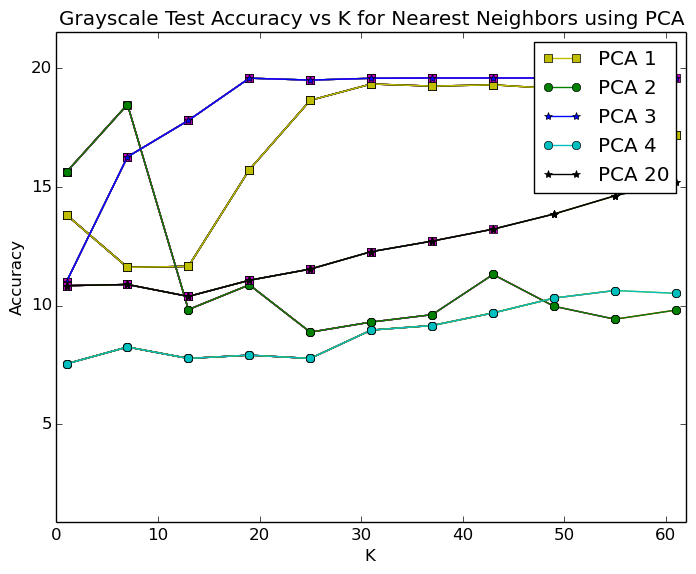
\includegraphics[width=.9\linewidth]{./plots/knn/majorityvote}
    	\caption{Performance of K-NN grayscale images using PCA with Majority Vote Rule}
	\label{fig:knn_vote}
\end{minipage}

\begin{minipage}{.5\textwidth}
  \centering
	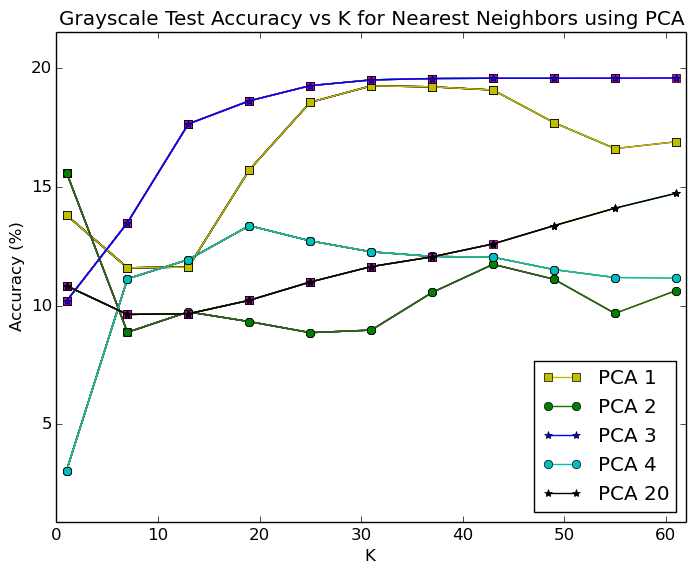
\includegraphics[width=0.9\linewidth]{./plots/knn/weighted}
    	\caption{Performance of K-NN grayscale images using PCA with Inverse-Distance Weighting}
	\label{fig:knn_weighted}
\end{minipage}
\end{figure}
\fi

\begin{figure}
\centering
	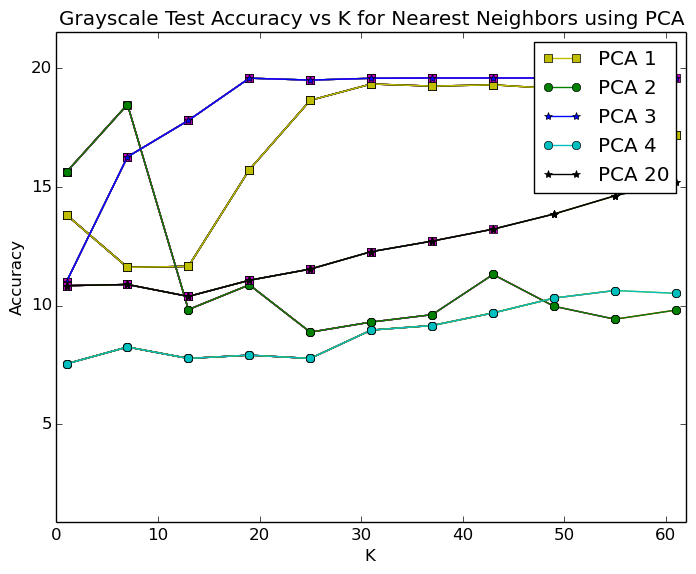
\includegraphics[width=0.8\linewidth]{./plots/knn/majorityvote}
    	\caption{Performance of K-NN grayscale images using PCA with Majority Vote Rule}
	\label{fig:knn_vote}
\end{figure}

\begin{figure}
\centering
	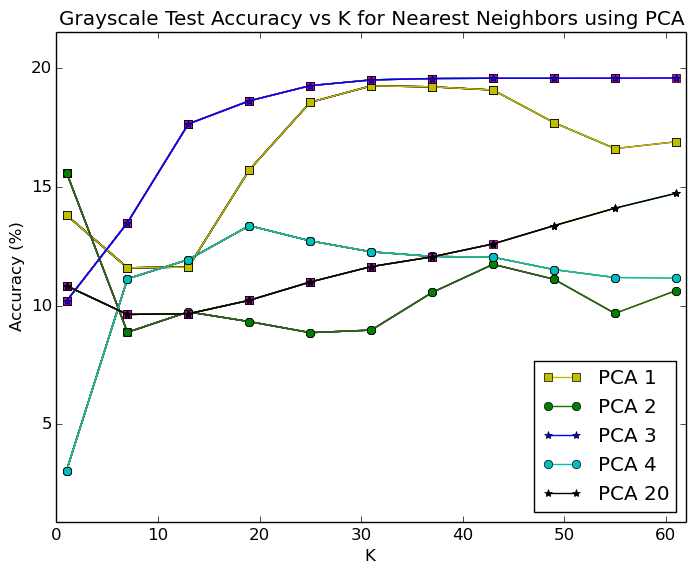
\includegraphics[width=0.8\linewidth]{./plots/knn/weighted}
    	\caption{Performance of K-NN grayscale images using PCA with Inverse-Distance Weighting}
	\label{fig:knn_weighted}
\end{figure}

\subsection{Conclusion}
For the majority vote nearest neighbour approach, using the top 3 dimensions from PCA in combination with $K=19$ neighbours produced the best results with $\approx 19.8\%$ while inverse-distance weighted nearest neighbours' optimal configuration was 3 dimensions from PCA in combination with $K=37$ neighbours yielding $\approx 18.2\%$. It is clear that K-NN is not a good technique for this domain due to the large intra-class variance.

\subsection{Discussion}
Since PCA was used to reduce the dimensions to 3 with over 76000 training examples it is extremely unlikely that distribution is not smooth (there are plenty of examples to fill out the 3-dimensional space with values ranging from 0 to 255), but rather that we are trying to cluster 10 classes in a 3-dimensional space in which it is probably the data model that is insufficient. Another interesting observation is that as the PCA dimension increased, the accuracy did not. This suggests that the data's variation does not contain information (as previously stated with large intra-class variance) thus violating PCA's principle assumption of "variance contains information". In this domain PCA is necessary for K-NN to make the computational burden feasible, however, PCA is a poor method to generate a predictive model as its underlying assumption is violated. Other techniques that could have been used in conjunction with K-NN would be bag of features to produce a vector descriptor of each example as a point in the K-NN space. The values indicate the weights had impact as the accuracies were not identical across majority and inverse-distance voting. Further configurations could be done using different distance metrics; however, we expect none to provide significant differences due to relying on PCA. 

\section{Support Vector Machines (Bag of Features)}

\subsection{Setup}
How to pose an image recognition task by using a SVM is non-trivial for many reasons: using the raw pixel data is too computationally expensive (with no guarantee on accuracy), so many algorithms extract features within the image and use these extracted features, with considerable fewer dimensions, as input to a clustering algorithm and define an image to be related to the clusters in which its features belong.  This algorithm is better known as "Bag of Words/Features" where we used a KMeans clustering algorithm and evaluated an image in two ways: using a count-per-cluster vector and a binary-cluster vector.  For example, if a provided image contains features lying close to centroids 1,2,1, and 4 the input to the SVM classifier would be [2,1,0,1] or [1,1,0,1] for the count and binary cluster vectors respectively.  We performed validation on the number of clusters in the set \{5,10,15,20,25,30,35,40,45\} in order to provide sufficient clusters to differentiate unique features and to limit the number of dimensions each example has as input to the SVM. KMeans was run until the change in distortion since the last iteration is less than or equal to $e^{-5}$. Additionally, to model complexity we tried using both a linear and quadratic SVM model with slack and a static penalization of 1.

\subsection{Configs \& Hand-Crafted Features}
We investigated the following features: histogram of oriented gradients (HoG), SURF, and SIFT; however, on preliminary investigation SIFT was performing approximately equal to random guessing and given that all the images are $32x32$ the "scale invariance" did not seem necessary so we omitted it for our tests.  We additionally tried using deskew in conjunction with HoG which helps align the image along the major vertical and horizontal axes.  We understand that this would have bigger impact for handwritten digits \cite{handwrittendigits} but decided to try it for SVHN as well.  We also noticed that SURF features were unable to be extracted for some examples (37773 and 13745 or 51.6\% and 52.8\% for training and testing datasets respectively) so we handled this in two ways: removing the examples, and randomly assigning a feature vector to it.  Note that $\approx 52\%$ is a large percentage of the datasets, and analogous with the results, we do not recommend using SURF for this domain.

Config 1--HoG\\
Config 2--HoG with Deskew\\
Config 3--SURF with Randomization\\
Config 4--SURF with Removal\\

\subsection{Results}
Figures~\ref{fig:clustercount} and \ref{fig:clusterbinary} show the results of using cluster-count and binary-cluster descriptors with the various feature configurations and number clusters using linear and quadratic SVMs. Cluster-count descriptors has the best observed performance; however, it seems that binary-cluster descriptors dominates in most of the configurations.

\begin{figure}
\centering
	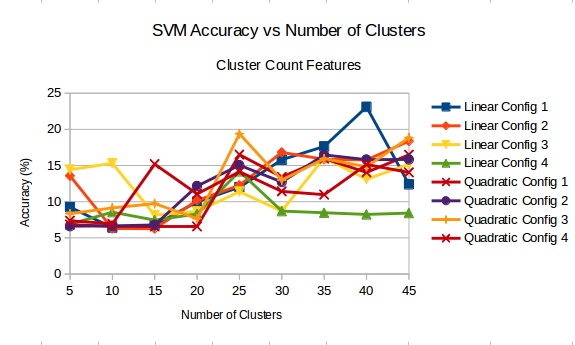
\includegraphics[width=0.9\linewidth]{./plots/svm/clustercount}
    	\caption{Performance of SVM using Bag of Features with KMeans Clustering with Cluster-Count Descriptors}
	\label{fig:clustercount}
\end{figure}

\begin{figure}
\centering
	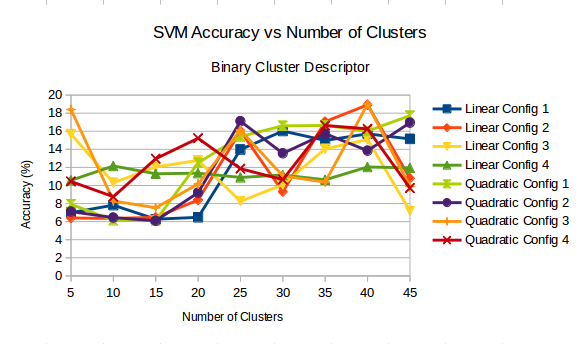
\includegraphics[width=0.9\linewidth]{./plots/svm/clusterbinary}
    	\caption{Performance of SVM using Bag of Features with KMeans Clustering with Binary Cluster Descriptors}
	\label{fig:clusterbinary}
\end{figure}

\subsubsection{Addendum}
After observing the training data we noticed that the images weren't quite cropped out as we expected.  There was a vast array of intra-class variations due to adjacent digits sneaking their way into the images.  We decided to run the best configuration one more time with trimming the width of every example.  We trim the width by \{4, 8, 12, 16, 20, 24, 28\} pixels total (\{2, 4, 8, 6, 10, 12, 14 \} pixels per side]) thus slicing out the middle section of the image leaving the height intact (because we read horizontally all adjacent digits appear to the left or right of the focus digit).  An example of such an image is depicted in figure~\ref{manydigits}.  The results of using this trimming version are in figure~\ref{fig:svmtrim}. Though there is a marginal increase in reducing image width by 4 pixels (total), it appears that overall reducing the width negatively affects the accuracy for our dataset.

\begin{figure}
\centering
	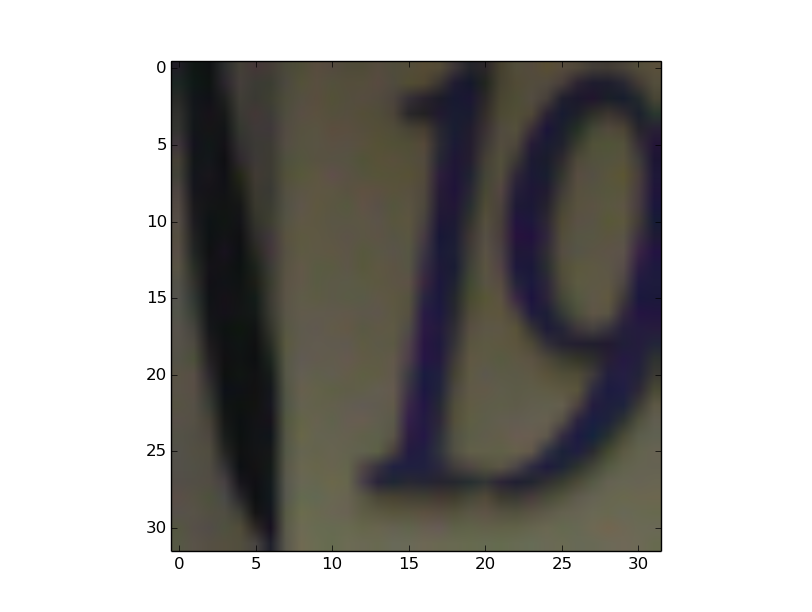
\includegraphics[scale=0.2]{./plots/manydigits}
    	\caption{An example of a training image with adjacent numbers intruding on the focus digit}
	\label{fig:manydigits}
\end{figure}

\begin{figure}
\centering
	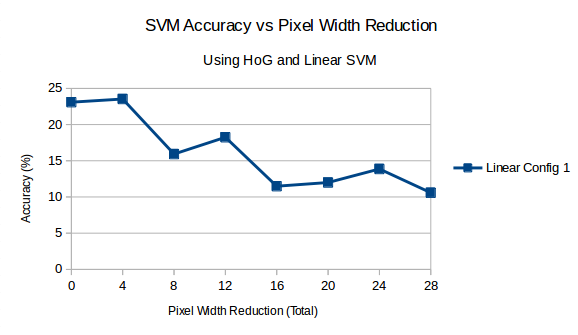
\includegraphics[width=0.8\linewidth]{./plots/svm/trim}
    	\caption{Reducing image width using Cluster-Counts with a Linear SVM and Config 1}
	\label{fig:svmtrim}
\end{figure}

\subsection{Sanity Check}
After running our algorithm with fairly poor results we decided to cross reference it with the MNIST dataset to determine the validity of our algorithm. First we ran the algorithm on the 10 digit class problem and still received very poor results. Then we decided to run it on a binary class problem using digits 0,7, and 2,3. We reached $\approx 94\%$ on the $0,7$ binary class problem and $\approx 82\%$ on the 2,3 problem using linear SVM with configuration 1. This helped reassure that our algorithm and pipeline (feature extraction, clustering, and evaluating cluster descriptors) was correct and also that SVM is not a good technique for this domain as its performance hindered on the more 'similar' digits (2,3).

\subsection{Conclusion}
Figure~\ref{fig:clustercount} shows that really none of the configurations (unlikely it is the SVM algorithm) are indicative of the classes represented in SVHN.  However, a linear SVM with configuration 1 (HoG with no deskew) using 40 clusters is the best with $\approx 23.1\%$.  Figure~\ref{fig:clusterbinary} has similar results with $\approx 19.0\%$ for a linear SVM with configurations 1 and 2 using 40 clusters.  Figure~\ref{fig:svmtrim} produced one slightly better result with $\approx 23.5\%$ accuracy using 32x28 images. From the methods we investigated the optimal strategy was HoG with reducing the width by 2 pixels on each side which slightly edged out the same configuration however keeping the images with original size. Future work would be to determine the optimal penalty (we used a static penalty of 1) and polynomial degree (though briefly investigating cubic showed no evidence in improvement and the linear SVM performed marginally better than the quadratic model).

\subsection{Discussion}
We expected trimming to produce better results given the obtrusion of extra digits in the images. It succeeded in improving the performance in one configuration but its marginal gains (0.5\%) at the expense of longer training time because you introduce one additional hyper-parameter (trim pixel length) which needs to be tuned together with the original hyper-parameters may not warrant its utilization. Though we did not carry out the investigation using SIFT we observed similar results in failing to extract features and approximately random guessing accuracy. SIFT and SURF detectors were ineffective as they failed to extract any feature on many examples (more than 50\%) and SIFT did not showcase its investigation as it added additional computational burden compared to SURF and the examples were on approximately the same scale. The results from SVM provide evidence that using hand-crafted features is likely not the optimal course of action. SIFT and SURF are unreliable while the added noise from environment and additional digits extremely hinders the performance of these hard-coded features. For cluster-count descriptors, the polynomial degree seems to favour linear models for the HoG and quadratic for SURF configurations while cluster-binary descriptors favour the quadratic model except for a few (in which the maximum was reached as well). There seems to be little correlation between cluster-count and binary cluster descriptors as they each outperform the other in different configurations.  This suggests that, given the hand-crafted features are accurate depictions (which they most likely are not), the SVM model is likely to not be either of these polynomials.

\section{Conclusion}
Convolutional neural networks prove their superiority over K-NN and SVM in computer visual tasks. While the best performances for K-NN and SVM reaches 19.8\% and 23.5\% respectively, the covolutional neural network far surpassed these other techniques with an 86\% performance. It is clear that the ability to learn features was crucial as, for example in SVM, the hand crafted features were not robust enough on the dataset, thus producing inaccurate results. Additionally, while K-NN perpetually struggles as the number of dimensions increase, raw pixel intensities were made seemingly meaningless. In addition, the vast intra-class variation made PCA's dependency on variation encoding information unfounded and so it was inaccurately projecting examples to a new dimensional space. Furthermore, convolutional neural networks can down sample these dimensions quickly using its hidden layers and, through back propagation, can automatically learn important features on the raw (colour) data. Though it was not a criteria to produce efficient and fast algorithms, it should be noted that neural networks (as well as SVMs) are fast in predicting (or inferring) future examples as the bulk of their work is done during training and the model could potentially be extracted and loaded as the user pleases. K-NN's ability to make timely predictions depends on the number of examples and their dimensions as all of its computation is done during the prediction stage (memory footprint aside).

\section*{Acknowledgments}

\small{
\nocite{*}
\bibliographystyle{plainnat}
\bibliography{research}
}
\end{document}